\section{Espacios normados}

\subsection{Cuestiones básicas}

\begin{ejercicio}
Probar que dos normas en un mismo espacio vectorial son equivalentes si, y sólo si, dan lugar a los mismos conjuntos acotados.
\begin{description}
    \item[$\Longrightarrow$)] Sea $X$ un espacio vectorial y $\|\cdot\|_1$ y $\|\cdot\|_2$ dos normas equivalentes en $X$. Entonces existen constantes $C_1, C_2 \in \bb{R}^+$ tales que
    \[
    C_1 \|x\|_1 \leq \|x\|_2 \leq C_2 \|x\|_1 \quad \forall x \in X
    \]
    Sea $A \subset X$ un conjunto acotado en la norma $\|\cdot\|_1$. Entonces existe $M \in \bb{R}^+$ tal que $\|x\|_1 \leq M$ para todo $x \in A$. Por lo tanto, para todo $x \in A$ se tiene que
    \[
    \|x\|_2 \leq C_2 \|x\|_1 \leq C_2 M
    \]
    y, por tanto, $A$ es acotado en la norma $\|\cdot\|_2$, con cota $C_2 M$. De manera análoga se demuestra que si $A$ es acotado en la norma $\|\cdot\|_2$, entonces también lo es en la norma $\|\cdot\|_1$.

    \item[$\Longleftarrow$)] Sea $X$ un espacio vectorial y $\|\cdot\|_1$ y $\|\cdot\|_2$ dos normas en $X$ que dan lugar a los mismos conjuntos acotados.
    
    Fijado $x \in X \setminus \{0\}$, consideremos el conjunto $A = \left\{\dfrac{x}{\|x\|_1}\right\}$. Este conjunto es acotado en la norma $\|\cdot\|_1$, y por hipótesis también lo es en la norma $\|\cdot\|_2$. Por tanto, existe $C_2 \in \bb{R}^+$ tal que
    \[
    \left\|\frac{x}{\|x\|_1}\right\|_2 \leq C_2
    \]
    y, por tanto, $\|x\|_2 \leq C_2 \|x\|_1$. De manera análoga se demuestra que existe $C_1' \in \bb{R}^+$ tal que $\|x\|_1 \leq C_1' \|x\|_2$. Considerando $C_1 = \nicefrac{1}{C_1'}$, se obtiene que:
    \[
    C_1 \|x\|_1 \leq \|x\|_2 \leq C_2 \|x\|_1
    \]

    Puesto que $x \in X \setminus \{0\}$ es arbitrario, y para $x = 0$ se tiene que $\|0\|_1 = \|0\|_2 = 0$, se concluye que las normas $\|\cdot\|_1$ y $\|\cdot\|_2$ son equivalentes.
\end{description}
\end{ejercicio}

\begin{ejercicio}
Si $X$ es un espacio normado, para $x \in X$ y $r \in \bb{R}^+$, denotamos por $B(x, r)$ a la bola cerrada de centro $x$ y radio $r$. Para $x, y \in X$ y $r, \rho \in \bb{R}^+$, probar las siguientes equivalencias:
\begin{enumerate}[label={\alph*)}]
    \item $B(x, r) \cap B(y, \rho) \neq \emptyset \sii \|x - y\| \leq r + \rho$
    
    La situación está ilustrada en la figura \ref{fig:interseccion_bolas}.
    \begin{figure}[htbp]
        \centering
        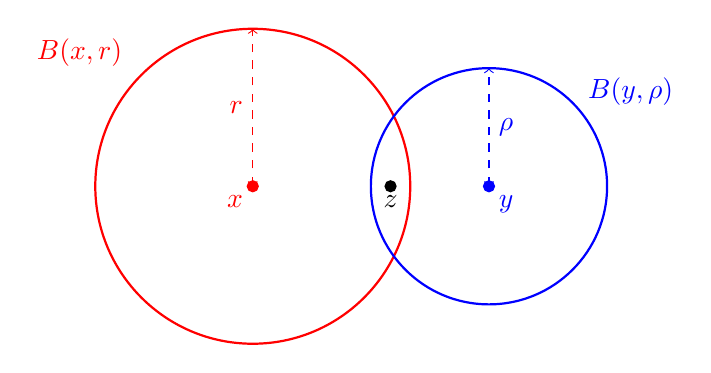
\begin{tikzpicture}
            \draw[thick, red] (0,0) circle (2cm);
            \draw[thick, blue] (3,0) circle (1.5cm);

            % Puntos de interés
            \filldraw[red] (0,0) circle (2pt) node[anchor=north east] {$x$};
            \filldraw[blue] (3,0) circle (2pt) node[anchor=north west] {$y$};
            \filldraw[black] (1.75,0) circle (2pt) node[anchor=north] {$z$};

            % Etiquetas de los radios
            \draw[<->, dashed, red] (0,0) -- (0,2) node[midway, left] {$r$};
            \draw[<->, dashed, blue] (3,0) -- (3,1.5) node[midway, right] {$\rho$};

            % Etiqueta de las bolas
            \node at (-2.2,1.7) [red] {$B(x,r)$};
            \node at (4.8,1.2) [blue] {$B(y,\rho)$};
        \end{tikzpicture}
        \caption{Intersección no vacía de dos bolas cerradas.}
        \label{fig:interseccion_bolas}
    \end{figure}

    Consideramos la distancia inducida por la norma: $d(x,y)=\|x-y\|,~\forall x,y\in X$.
    \begin{description}
        \item[$\Longrightarrow)$]
        Sea $z \in B(x, r) \cap B(y, \rho)$. Por definición de bola cerrada, $d(x, z) \leq r$ y $d(y, z) \leq \rho$. Entonces, por la desigualdad triangular:
        \begin{equation*}
            \|x - y\| = d(x, y) \leq d(x, z) + d(z, y) \leq r + \rho
        \end{equation*}

        \item[$\Longleftarrow)$]
        Suponemos $\|x - y\| \leq r + \rho$, y buscamos $z \in B(x, r) \cap B(y, \rho)$.
        
        Si $x = y$, basta tomar $z = x$, ya que $\|x - x\| = 0 \leq r$ y $\|x - y\| = 0 \leq \rho$.
        
        Supongamos por tanto que $x \neq y$. Consideramos un punto del segmento que une $x$ e $y$, definido por $z := \lambda x + (1 - \lambda)y$ para $\lambda \in [0, 1]$. Estudiamos las condiciones para que pertenezca a ambas bolas:
        \begin{equation*}\begin{split}
            z \in B(x, r) &\iff \|z - x\| \leq r \iff \|(1 - \lambda)(y - x)\| = (1 - \lambda)\|x - y\| \leq r \\
            &\iff 1 - \frac{r}{\|x - y\|} \leq \lambda \\
            z \in B(y, \rho) &\iff \|z - y\| \leq \rho \iff \|\lambda(x - y)\| = \lambda \|x - y\| \leq \rho \\
            &\iff \lambda \leq \frac{\rho}{\|x - y\|}
        \end{split}\end{equation*}

        Por tanto, buscamos $\lambda \in [0, 1]$ que satisfaga:
        \begin{equation*}
            1 - \frac{r}{\|x - y\|} \leq \lambda \leq \frac{\rho}{\|x - y\|}
        \end{equation*}
        Dicho valor existe en $\bb{R}$ si y solo si el extremo inferior es menor o igual que el superior:
        \begin{equation*}
            1 - \frac{r}{\|x - y\|} \leq \frac{\rho}{\|x - y\|} \iff \|x - y\| - r \leq \rho \iff \|x - y\| \leq r + \rho
        \end{equation*}
        lo cual es cierto por hipótesis. Además, como $r, \rho > 0$, se tiene $1 - \frac{r}{\|x-y\|} < 1$ y $\frac{\rho}{\|x-y\|} > 0$. Tomando, por ejemplo,
        \begin{equation*}
            \lambda = \max\left\{0, \, 1 - \frac{r}{\|x - y\|}\right\}
        \end{equation*}
        se comprueba que $\lambda \in [0, 1]$ y cumple ambas desigualdades. Por tanto, existe $z \in B(x, r) \cap B(y, \rho)$, concluyendo que la intersección no es vacía.
    \end{description}
    \item $B(x, r) \subset B(y, \rho) \sii \|x - y\| \leq \rho - r$
    
    La situación está ilustrada en la figura \ref{fig:inclusion_bolas}.
    \begin{figure}[htbp]
        \centering
        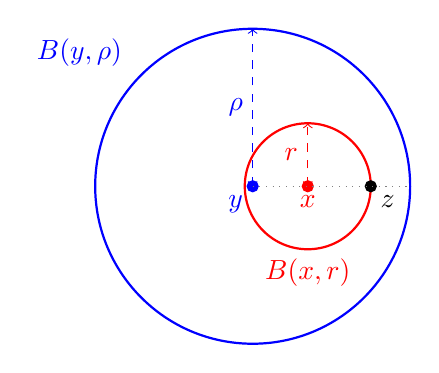
\begin{tikzpicture}
            % Bola mayor exterior B(y, rho)
            \draw[thick, blue] (0,0) circle (2cm);
            % Bola menor interior B(x, r)
            \draw[thick, red] (0.7,0) circle (0.8cm);

            % Puntos de interés
            \filldraw[blue] (0,0) circle (2pt) node[anchor=north east] {$y$};
            \filldraw[red] (0.7,0) circle (2pt) node[anchor=north] {$x$};
            \filldraw[black] (1.5,0) circle (2pt) node[anchor=north west] {$z$};

            % Etiquetas de los radios
            \draw[<->, dashed, blue] (0,0) -- (0,2) node[midway, left] {$\rho$};
            \draw[<->, dashed, red] (0.7,0) -- (0.7,0.8) node[midway, left] {$r$};

            % Semirrecta que ilustra la elección de z
            \draw[dotted, gray] (0,0) -- (2,0);

            % Etiqueta de las bolas
            \node at (-2.2,1.7) [blue] {$B(y,\rho)$};
            \node at (0.7,-1.1) [red] {$B(x,r)$};
        \end{tikzpicture}
        \caption{Inclusión de la bola $B(x,r)$ en la bola $B(y,\rho)$.}
        \label{fig:inclusion_bolas}
    \end{figure}

    \begin{description}
        \item[$\Longrightarrow)$]
        Supuesto $x = y$, tenemos que $B(x, r) \subset B(x, \rho)$ si y solo si $r \leq \rho$, lo cual equivale a $\|x - y\| = 0 \leq \rho - r$. Supongamos por tanto que $x \neq y$.

        Consideramos el punto:
        \begin{equation*}
            z = x + r \frac{x - y}{\|x - y\|}
        \end{equation*}
        Calculamos su distancia a $x$:
        \begin{equation*}
            \|z - x\| = \left\| r \frac{x - y}{\|x - y\|} \right\| = r \frac{\|x - y\|}{\|x - y\|} = r \leq r
        \end{equation*}
        Por tanto, $z \in B(x, r)$. Como por hipótesis $B(x, r) \subset B(y, \rho)$, se deduce que $z \in B(y, \rho)$, es decir, $\|z - y\| \leq \rho$.

        Calculamos explícitamente $\|z - y\|$:
        \begin{align*}
            \|z - y\| &= \left\| x - y + r \frac{x - y}{\|x - y\|} \right\| = \left\| (x - y)\left(1 + \frac{r}{\|x - y\|}\right) \right\| \\
            &= \left(1 + \frac{r}{\|x - y\|}\right)\|x - y\| = \|x - y\| + r
        \end{align*}
        Como $\|z - y\| \leq \rho$, obtenemos directamente:
        \begin{equation*}
            \|x - y\| + r \leq \rho \iff \|x - y\| \leq \rho - r
        \end{equation*}

        \item[$\Longleftarrow)$]
        Supongamos que $\|x - y\| \leq \rho - r$. Sea $z \in B(x, r)$ arbitrario, es decir, $\|z - x\| \leq r$. Veamos que $z \in B(y, \rho)$:
        \begin{equation*}
            \|z - y\| \leq \|z - x\| + \|x - y\| \leq r + (\rho - r) = \rho
        \end{equation*}
        Por tanto, $z \in B(y, \rho)$, demostrando la inclusión $B(x, r) \subset B(y, \rho)$.
    \end{description}
\end{enumerate}
\end{ejercicio}

\begin{ejercicio}
Sea $X$ un espacio de Banach y $\{B_n\}$ una sucesión de bolas cerradas en $X$, que sea decreciente, es decir, $B_{n+1} \subset B_n$ para todo $n \in \bb{N}$. Probar que $\bigcap\limits_{n=1}^\infty B_n \neq \emptyset$.\\

En vistas a emplear la propiedad de completitud de $X$, buscamos una sucesión de Cauchy $\{x_n\}$ con $x_n \in B_n$ para todo $n \in \bb{N}$. Sabiendo que $X$ es completo, la sucesión $\{x_n\}$ convergerá a un punto $x \in X$ que, por ser límite de una sucesión de puntos de $B_n$ conjunto cerrado, pertenecerá a $B_n$ para todo $n \in \bb{N}$, y por tanto a la intersección $\bigcap\limits_{n=1}^\infty B_n$. Formalicemos esta idea.

Fijado $n \in \bb{N}$, sea $B_n = B(x_n, r_n)$, con $x_n \in X$ y $r_n \in \bb{R}^+$. Como $\{B_n\}$ es decreciente, se tiene que $B_{n+1} \subset B_n$, y por lo demostrado en el ejercicio anterior, se deduce que $\|x_{n+1} - x_n\| \leq r_n - r_{n+1}$. De esta idea, deducimos que $\{r_n\}$ es una sucesión decreciente de números reales minorada por cero. Por la caracterización del ínfimo por sucesiones, $\{r_n\}$ converge a un número real $R\in \bb{R}^+_0$.
\begin{equation*}
    \{r_n\} \longrightarrow R \geq 0
\end{equation*}

Asímismo, y en vistas de demostrar que $\{x_n\}$ es de Cauchy, fijados $m, n \in \bb{N}$ con $m > n$, hemos de calcular $\|x_m - x_n\|$. Por la desigualdad triangular, tenemos que:
\begin{equation*}
    \|x_m - x_n\| \leq \sum_{k=n}^{m-1} \|x_{k+1} - x_k\| \leq \sum_{k=n}^{m-1} (r_k - r_{k+1}) = r_n - r_m
\end{equation*}

Distinguimos ahora en función del valor de $R$.
\begin{description}
    \item[Si $R=0$:] Entonces, por definición de convergencia de $\{r_n\}$, tenemos que:
    \begin{equation*}
        \forall \varepsilon > 0, \exists n_0 \in \bb{N} : n \geq n_0 \implies r_n < \varepsilon
    \end{equation*}

    Por tanto, fijado $\veps\in \bb{R}^+$, consideramos el valor de $n_0$ dado por la convergencia de $\{r_n\}$. Para cualesquiera $m, n \in \bb{N}$ con $m > n \geq n_0$, se tiene que:
    \begin{equation*}
        \|x_m - x_n\| \leq r_n - r_m < r_n < \varepsilon
    \end{equation*}

    Por tanto, $\{x_n\}$ es una sucesión de Cauchy, y como $X$ es completo, $\{x_n\}$ converge a un punto $x \in X$.
    \begin{equation*}
        \{x_n\} \longrightarrow x \in X
    \end{equation*}

    Veamos ahora que $x \in \bigcap\limits_{n=1}^\infty B_n$. Fijado $n \in \bb{N}$, como $B_n$ es cerrado y $\{x_m\}_{m\geq n} \subset B_n$, se tiene que $x \in B_n$, puesto que el límite de una sucesión de puntos de un conjunto cerrado pertenece al conjunto. Por tanto, $x \in B_n$ para todo $n \in \bb{N}$, y por tanto $x \in \bigcap\limits_{n=1}^\infty B_n$.

    \item[Si $R>0$:] En este caso, la sucesión $\{r_n\}$ converge a un número real positivo. Podemos no obstante definir una nueva sucesión de bolas cerradas $\{B_n'\}$, con $B_n' = B(x_n, r_n - R)$, que cumpla la hipótesis del caso anterior.
    
    En primer lugar, veamos que es decreciente. Fijados $n \in \bb{N}$, veamos que:
    \begin{equation*}
        B_{n+1}' = B(x_{n+1}, r_{n+1} - R) \subset B(x_n, r_n - R) = B_n'
    \end{equation*}

    Tenemos que:
    \begin{equation*}
        \|x_{n+1} - x_n\| \leq r_n - r_{n+1} = (r_n - R) - (r_{n+1} - R)
    \end{equation*}

    Aplicando el ejercicio anterior, se deduce que $B_{n+1}' \subset B_n'$, y por tanto $\{B_n'\}$ es decreciente. Además, como $\{r_n - R\}$ converge a cero, podemos aplicar el caso anterior para deducir que:
    \begin{equation*}
        \bigcap_{n=1}^\infty B_n' \neq \emptyset
    \end{equation*}

    Por tanto, existe $x \in X$ tal que $x \in B_n'$ para todo $n \in \bb{N}$. Como $B_n' \subset B_n$ para todo $n \in \bb{N}$, se concluye que $x \in B_n$ para todo $n \in \bb{N}$, y por tanto $x \in \bigcap\limits_{n=1}^\infty B_n$.
\end{description}
\end{ejercicio}

\begin{ejercicio}
Probar que, si $X$ es un espacio normado, para cualesquiera $x, y \in X \setminus \{0\}$ se verifica la siguiente desigualdad:
\[
\left\| \frac{x}{\|x\|} - \frac{y}{\|y\|} \right\| \leq \frac{2\|x - y\|}{\max\{\|x\|, \|y\|\}}
\]

    Supongamos sin pérdida de generalidad que $\|y\| \leq \|x\|$, puesto que en caso contrario, intercambiando $x$ e $y$, se obtiene la misma desigualdad. Entonces, $\max\{\|x\|, \|y\|\} = \|x\|$. Sumamos y restamos $\dfrac{y}{\|x\|}$ en el primer miembro de la desigualdad:
    \begin{equation*}
        \left\| \frac{x}{\|x\|} - \frac{y}{\|y\|} \right\| = \left\| \frac{x}{\|x\|} - \frac{y}{\|x\|} + \frac{y}{\|x\|} - \frac{y}{\|y\|} \right\| \leq \left\| \frac{x - y}{\|x\|} \right\| + \left\| \dfrac{y}{\|x\|} - \dfrac{y}{\|y\|} \right\|
    \end{equation*}

    Respecto al primer sumando, por homogeneidad de la norma, se tiene que:
    \begin{equation*}
        \left\| \frac{x - y}{\|x\|} \right\| = \frac{\|x - y\|}{\|x\|}
    \end{equation*}

    Respecto al segundo sumando, factorizamos $y$ y aplicamos la desigualdad triangular inversa:
    \begin{equation*}
        \left\| \dfrac{y}{\|x\|} - \dfrac{y}{\|y\|} \right\| = \left\|y\right\| \left| \frac{1}{\|x\|} - \frac{1}{\|y\|} \right| = \|y\| \, \frac{|\|y\| - \|x\||}{\|x\| \, \|y\|} \leq \|y\| \,  \frac{\|x - y\|}{\|x\| \, \|y\|} = \frac{\|x - y\|}{\|x\|}
    \end{equation*}

    Por tanto, se concluye que:
    \begin{equation*}
        \left\| \frac{x}{\|x\|} - \frac{y}{\|y\|} \right\| \leq \frac{\|x - y\|}{\|x\|} + \frac{\|x - y\|}{\|x\|} = \frac{2\|x - y\|}{\|x\|} = \frac{2\|x - y\|}{\max\{\|x\|, \|y\|\}}
    \end{equation*}
\end{ejercicio}

\begin{ejercicio}
Sean $A$ y $B$ subconjuntos no vacíos de un espacio normado. Probar las siguientes afirmaciones:
\begin{enumerate}[label={\alph*)}]
    \item Si $A$ es abierto, entonces $A + B$ es abierto.
    
    Recordamos que:
    \begin{equation*}
        A + B = \{a + b : a \in A, b \in B\}
    \end{equation*}

    \begin{description}
        \item[Opción 1] Si $x \in A + B$, entonces existen $a \in A$ y $b \in B$ tales que $x = a + b$. Como $A$ es abierto, existe $r \in \bb{R}^+$ tal que $U(a, r) \subset A$. Consideremos la bola abierta $U(x, r)$, y tenemos que demostrar que $U(x, r) \subset A + B$. Sea $y \in U(x, r)$ arbitrario, y escribamos $y = (y -b) + b$. Veamos que $y - b \in U(a, r)$:
        \begin{equation*}
            \|y - b - a\| = \|y - (a + b)\| = \|y - x\| < r
        \end{equation*}
        Por tanto, $y - b \in U(a, r) \subset A$, y como $b \in B$, se puede concluir que $y = (y - b) + b \in A + B$. Por tanto, $U(x, r) \subset A + B$, y como $x \in A + B$ es arbitrario, se concluye que $A + B$ es abierto.
        
        \item[Opción 2] Tenemos que:
        \begin{equation*}
            A + B = \bigcup_{b \in B} (A + b)
        \end{equation*}

        Fijado $b \in B$, consideremos la siguiente aplicación:
        \Func{T_b}{X}{X}{x}{x + b}

        Esta aplicación, traslación por $b$, es un homeomorfismo en $X$, y por tanto $A + b=T_b(A)$ es abierto. Como $A + B$ es la unión de abiertos, se concluye que $A + B$ es abierto.
    \end{description}
    \item Si $A$ es compacto y $B$ es cerrado, entonces $A + B$ es cerrado.
    
    Consideramos una sucesión $\{x_n\}$ en $A + B$ que converge a un punto $x \in X$. Queremos ver que $x \in A + B$. Para cada $n \in \bb{N}$, existen $a_n \in A$ y $b_n \in B$ tales que:
    \begin{equation*}
        x_n = a_n + b_n
    \end{equation*}

    Como $A$ es compacto\footnote{Notemos que no estamos empleando el concepto general de compacidad, sino su equivalente para espacios métricos visto en Análisis Matemático I.}, existe una parcial $\{a_{\sigma(n)}\}$ de $\{a_n\}$ que converge a un punto $a \in A$. Por tanto, para cada $n\in \bb{N}$, tenemos que:
    \begin{equation*}
        b_{\sigma(n)} = x_{\sigma(n)} - a_{\sigma(n)} \in B
    \end{equation*}

    Además, como $\{x_n\}\to x$ y $\{a_{\sigma(n)}\}\to a$ y toda parcial de una sucesión convergente converge al mismo límite, se concluye que $\{b_{\sigma(n)}\}\to x - a$. Como $B$ es cerrado, se deduce que $x - a \in B$, y por tanto $x = a + (x - a) \in A + B$. Por tanto, $A + B$ es cerrado.
\end{enumerate}
Dar un ejemplo en el que $A$ y $B$ sean cerrados pero $A + B$ no sea cerrado.\\


Notemos que hemos de buscar un ejemplo en el que $A$ no sea compacto, ya que de lo contrario, por el resultado anterior, $A + B$ sería cerrado. En particular, podemos buscar un ejemplo. En $\bb{R}^n$, vimos que ser compacto es equivalente a ser cerrado y acotado, luego hemos de buscar dos conjuntos cerrados pero no acotados. Veamos dos ejemplos:
\begin{enumerate}
    \item Consideramos el espacio normado $\bb{R}$, y sean:
    \begin{equation*}
        A = \bb{Z} \quad \text{y} \quad B = \left\{n + \frac{1}{n+1} : n \in \bb{N}\right\}
    \end{equation*}

    Tenemos que $A$ y $B$ son cerrados, pero veamos que $A + B$ no es cerrado. Consideremos la sucesión $\{x_n\}$ definida por:
    \begin{equation*}
        x_n = -n + \left(n + \frac{1}{n+1}\right) = \frac{1}{n+1} \in A + B
    \end{equation*}
    La sucesión $\{x_n\}$ converge a $0$, y veamos que $0 \notin A + B$.
    \begin{itemize}
        \item Supongamos que $0 \in A + B$. Entonces, existen $a \in A=\bb{Z}$ y $b \in B$ tales que $0 = a + b$. Como $b\in B$, existe $n \in \bb{N}$ tal que $b = n + \frac{1}{n+1}$, luego:
        \begin{equation*}
            0 = a + b = a + n + \frac{1}{n+1} \implies -(a + n) = \frac{1}{n+1}
        \end{equation*}

        Como $a + n \in \bb{Z}$, se deduce que $-(a + n) \in \bb{Z}$. No obstante, tenemos que:
        \begin{equation*}
            0 < \frac{1}{n+1} < 1
        \end{equation*}
        lo cual es una contradicción, ya que ningún número entero puede ser igual a un número estrictamente positivo menor que $1$. Por tanto, $0 \notin A + B$.
    \end{itemize}
    Por tanto, $A + B$ no es cerrado.
    \item Consideramos el espacio normado $\bb{R}^2$, y sean:
    \begin{equation*}
        A = \bb{R}^+ \times \{0\} \quad \text{y} \quad B = \left\{(x, y) \in \bb{R}^2 : y = e^x\right\}
    \end{equation*}
    \begin{figure}
        \centering
        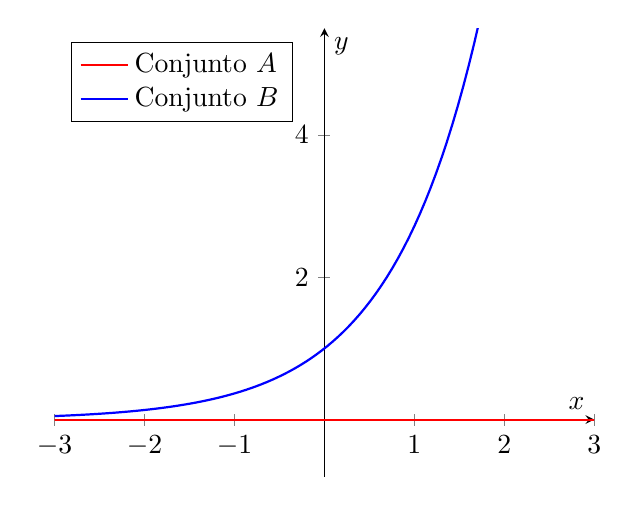
\begin{tikzpicture}
            \begin{axis}[
                axis lines = middle,
                xlabel = {$x$},
                ylabel = {$y$},
                xmin = -3, xmax = 3,
                ymin = -0.8, ymax = 5.5,
                legend pos = north west,       % Posición: north west, north east, south west, etc.
                legend cell align = {left},    % Alineación del texto en la leyenda
                samples = 100,                 % Calidad de la curva exponencial
                domain = -3:3
            ]
                % Conjunto A (eje o semieje horizontal)
                \addplot[thick, red, domain=-5:5] {0};
                \addlegendentry{Conjunto $A$}

                % Conjunto B (curva exponencial)
                \addplot[thick, blue, domain=-3:3] {exp(x)};
                \addlegendentry{Conjunto $B$}
                
            \end{axis}
        \end{tikzpicture}
        \caption{Conjuntos $A$ y $B$ en $\mathbb{R}^2$.}
        \label{fig:conjuntos_A_B}
    \end{figure}
    Los conjuntos $A$ y $B$ están mostrados en la figura \ref{fig:conjuntos_A_B}. El conjunto $A$ es trivialmente cerrado, y el conjunto $B$ es cerrado porque es la gráfica de una función continua. No obstante, tenemos que $A + B=\bb{R} \times \bb{R}^+$, que no es cerrado, ya que su frontera $\bb{R} \times \{0\}$ no está incluida en el conjunto.
\end{enumerate}
\end{ejercicio}

\subsection{Ejemplos}

\begin{ejercicio}
En el espacio vectorial $C^1\left[0, 1\right]$ formado por todas las funciones de clase $C^1$ en el intervalo $\left[0, 1\right]$, con valores en $\bb{K}$, se define
\[
\|f\| = |f(0)| + \max\left\{ |f'(t)| : t \in \left[0, 1\right] \right\} \quad \forall f \in C^1\left[0, 1\right]
\]
Probar que de esta forma se obtiene una norma completa en $C^1\left[0, 1\right]$.
\end{ejercicio}

\begin{ejercicio}
En el espacio $\bb{K}^{\bb{N}}$ de todas las sucesiones de escalares, se considera el subespacio definido por
\[
X = \left\{ x \in \bb{K}^{\bb{N}} : \sum_{n=1}^\infty \frac{|x(n)|}{n} < \infty \right\}
\]
y se define una norma en $X$ escribiendo
\[
\|x\| = \sum_{n=1}^\infty \frac{|x(n)|}{n} \quad \forall x \in X
\]
Probar que con esta norma, $X$ es un espacio de Banach.
\end{ejercicio}

\begin{ejercicio}
Dar un ejemplo de una sucesión $\{x_n\}$ en $\ell_1$:
\begin{enumerate}[label={\alph*)}]
    \item que converja a cero en $\ell_\infty$ pero no esté acotada en $\ell_2$.
    \item que converja a cero en $\ell_2$ pero no esté acotada en $\ell_1$.
\end{enumerate}
\end{ejercicio}

\begin{ejercicio}
Para cada $n \in \bb{N}$ y cada $t \in \left[0, 1\right]$ se define $f_n(t) = t^n - t^{n+1}$ y $g_n(t) = t^n - t^{2n}$. Estudiar la convergencia de las sucesiones $\{f_n\}$ y $\{g_n\}$:
\begin{enumerate}[label={\alph*)}]
    \item en el espacio de Banach $C\left[0, 1\right]$.
    \item en el espacio de Banach $L_p$, con $1 \leq p < \infty$.
\end{enumerate}
\end{ejercicio}

\begin{ejercicio}
Se consideran los conjuntos
\[
U = \{x \in c_0 : |x(n)| < 1 \;\; \forall n \in \bb{N}\} \quad \text{y} \quad V = \{x \in \ell_\infty : |x(n)| < 1 \;\; \forall n \in \bb{N}\}
\]
Probar que $U$ es abierto en $c_0$ pero $V$ no es abierto en $\ell_\infty$.
\end{ejercicio}

\subsection{Operadores y funcionales}

\begin{ejercicio}
Sean $X$ e $Y$ espacios normados y $T: X \longrightarrow Y$ un operador lineal. Supongamos que, para toda sucesión $\{x_n\}$ de vectores de $X$ tal que $\{x_n\} \to 0$, se tiene que la sucesión $\{T(x_n)\}$ está acotada. Probar que $T$ es continuo.
\end{ejercicio}

\begin{ejercicio}
En cada uno de los siguientes casos, probar que la aplicación $f \mapsto T(f)$ es un operador lineal continuo de $C\left[0, 1\right]$ en sí mismo, y calcular su norma:
\begin{enumerate}[label={\roman*)}]
    \item $\left[T(f)\right](t) = \int_{0}^t f(s)\,ds \quad \forall t \in \left[0, 1\right], \; \forall f \in C\left[0, 1\right]$
    \item $\left[T(f)\right](t) = t^2 f(0) \quad \forall t \in \left[0, 1\right], \; \forall f \in C\left[0, 1\right]$
    \item $\left[T(f)\right](t) = f(t^2) \quad \forall t \in \left[0, 1\right], \; \forall f \in C\left[0, 1\right]$
\end{enumerate}
\end{ejercicio}

\begin{ejercicio}
Fijada $g \in L_\infty\left[0, 1\right]$, probar que, para $1 \leq p \leq \infty$, la aplicación $f \mapsto fg$ es un operador lineal continuo de $L_p\left[0, 1\right]$ en sí mismo, y calcular su norma.
\end{ejercicio}

\begin{ejercicio}
Se considera el espacio normado $X = \{f \in C\left[0, 1\right] : f(\nicefrac{1}{2}) = 0\}$, con la norma inducida por $C\left[0, 1\right]$, y el funcional lineal $\varphi: X \longrightarrow \bb{K}$ definido por
\[
\varphi(f) = \int_{0}^1 f(t)\,dt \quad \forall f \in X
\]
Probar que es continuo y calcular su norma.
\end{ejercicio}

\begin{ejercicio}
Sea $\{e_n\}$ la base de vectores unidad de $c_0$. Probar que, para $f \in c_0^*$, las siguientes afirmaciones son equivalentes:
\begin{enumerate}[label={\Roman*)}]
    \item La función $|f|$ tiene máximo en la esfera unidad de $c_0$.
    \item Existe $m \in \bb{N}$ tal que $f(e_n) = 0$ para todo $n \in \bb{N}$ con $n \geq m$.
\end{enumerate}
Dar un ejemplo en el que no se verifiquen estas afirmaciones.
\end{ejercicio}

\begin{ejercicio}
Para $1 < p < \infty$, cualquier funcional lineal definido en $\ell_p$ alcanza su norma.
\end{ejercicio}

\begin{ejercicio}
Encontrar un operador lineal acotado de $\ell_2$ en otro espacio de Banach que no alcance su norma (esto es, que el supremo que define su norma no sea un máximo).
\end{ejercicio}

\subsection{Operaciones con espacios normados}

\begin{ejercicio}
Dado un espacio normado $X$, sean $f, g \in X^* \setminus \{0\}$. Probar que los espacios normados $\ker f$ y $\ker g$, ambos con la norma inducida por $X$, son isomorfos. Dar un ejemplo en el que dichos espacios no sean isométricamente isomorfos.
\end{ejercicio}

\begin{ejercicio}
Si $X$ e $Y$ son espacios normados y $Z = X \times Y$ es el espacio normado producto, probar que $Z^*$ es isomorfo al espacio de Banach producto $X^* \times Y^*$.
\end{ejercicio}

\begin{ejercicio}
En el espacio normado cociente $\ell_\infty / c_0$, calcular la norma cociente $\|x + c_0\|$, para cada $x \in \ell_\infty$.
\end{ejercicio}

\begin{ejercicio}
En el espacio de Banach $C\left[0, 1\right]$ se considera el subespacio
\[
M = \left\{g \in C\left[0, 1\right] : g(t) = 0 \;\; \forall t \in \left[0, \nicefrac{1}{2}\right]\right\}
\]
Probar que $M$ es cerrado en $C\left[0, 1\right]$, y calcular la norma cociente $\|f + M\|$ para cada $f \in C\left[0, 1\right]$.
\end{ejercicio}

\begin{ejercicio}
Para $1 \leq p < \infty$, se consideran los subespacios de $L_p$ definidos por
\[
M = \left\{f \in L_p : f(t) = 0 \text{ c.t.p. } t \in \left[0, \nicefrac{1}{2}\right]\right\}
\]
\[
Z = \left\{f \in L_p : f(t) = 0 \text{ c.t.p. } t \in \left[\nicefrac{1}{2}, 1\right]\right\}
\]
Probar que $L_p = M \oplus Z$, suma topológica directa. Deducir que $L_p$ es isomorfo al espacio de Banach producto $L_p \times L_p$.
\end{ejercicio}

\subsection{Espacios de dimensión finita}

\begin{ejercicio}
Sean $X$ e $Y$ espacios normados y supongamos que $Y$ tiene dimensión finita. Probar que todo operador lineal sobreyectivo $T: X \longrightarrow Y$ es una aplicación abierta.
\end{ejercicio}

\begin{ejercicio}
Sea $f: \left[0, 1\right] \longrightarrow \bb{K}$ una función continua, y supongamos que existen dos sucesiones de escalares $\{a_n\}$ y $\{b_n\}$ tales que:
\[
\lim\limits_{n \to \infty} \int_{0}^1 |f(t) - a_n e^t - b_n e^{-t}|^4\,dt = 0
\]
Probar que existen $a, b \in \bb{K}$ tales que $f(t) = a\,e^t + b\,e^{-t}$ para todo $t \in \left[0, 1\right]$.
\end{ejercicio}

\begin{ejercicio}
Probar que, para cada $N \in \bb{N}$, existe una constante $C_N \in \bb{R}^+$ verificando que, si $P$ es un polinomio de grado $N$ con coeficientes complejos, se tiene:
\[
\sum_{k=0}^N |P(k)| \leq C_N \int_{0}^1 |P(t)|\,dt
\]
\end{ejercicio}

\begin{ejercicio}
Sea $X$ un espacio normado y $M$ un subespacio de dimensión finita de $X$, tal que $M \neq X$. Probar que existe $x \in X$ tal que $\|x\| = d(x, M) = 1$. Deducir que, si $X$ tiene dimensión infinita, existe una sucesión $\{x_n\}$ en la esfera unidad de $X$, tal que $\|x_n - x_m\| \geq 1$ para cualesquiera $n, m \in \bb{N}$ con $m \neq n$.
\end{ejercicio}

\begin{ejercicio}
En el espacio de Banach $C\left[0, 1\right]$ se considera el subespacio
\[
M = \left\{f \in C\left[0, 1\right] : \int_{0}^1 f(t)\,dt = 0\right\}
\]
Probar que $M$ es proximinal en $C\left[0, 1\right]$.
\end{ejercicio}